\documentclass[10.5pt,letter]{exam}
\usepackage{graphicx,xcolor}
\usepackage{amsmath,amssymb,amsfonts}
\usepackage{array}

\newcommand{\ans}[1]{\textcolor{blue}{#1}}
\begin{document}

\begin{center}
    {\bf AERO 422 Fall 2021\\
    Homework 5} \\
    Box your final answers for all questions.
\end{center}

\begin{questions}
    \begin{figure}[hbt!]
        \centering
        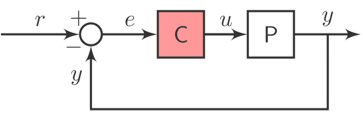
\includegraphics[width=0.4\textwidth]{AERO_422_HW5_P1.png}
        \caption{Standard negative unity feedback system}
        \label{fig:CLsys}
    \end{figure}
\question[3] A proposed hypersonic plane would climb to 100,000 feet, fly 3,800 miles per hour, and cross
the Pacific in 2 hours. Control of the aircraft can be represented by the system in Figure \ref{fig:CLsys}, with $C(s)=1$ and $$P(s) = \frac{12s+60}{s^3+(a+1)s^2+as}.$$
For this system, taking $a$ to be the parameter of interest, determine the Evans form representation
of the closed-loop characteristic equation.\\
\ans{Solution in other document.}

\question[3] In Figure \ref{fig:CLsys}, assume a proportional-only controller with gain $K$.
Use MATLAB to generate the root locus plot for each one of the following plant transfer function as the proportional gain $K$ varies from 0 to $\infty$. 
\begin{parts}
\part $P(s) = \big(s^2+2s+10\big)\big(s^5+9s^4+40.25s^3+106.5s^2+141.75s+67.5\big)^{-1}$
\part $P(s) = \big(s^2+5s/6+1/3\big)\Big(s^3 \big(s^2+6s+16\big)\Big)^{-1}$
\end{parts}
\ans{Solution in other document.}

\question In Figure \ref{fig:CLsys}, assume a proportional-only controller, i.e. $C(s)=K$, and $$ P(s) = \frac{1}{(s^2+2s+2)(s+1)} .$$
\begin{parts}
    \part[9]
    Sketch the Root Locus (by hand) for $0 \leq K < \infty$. 
    Go through the entire seven-step process, and state the answers for each step. Do not skip
    any steps. If a step is not required, provide a complete explanation for why it does not apply.\\
    \ans{Solution in other document.}
    \part[1] Use MATLAB to generate the root locus, and verify your results.
    \begin{figure}[hbt!]
        \centering
        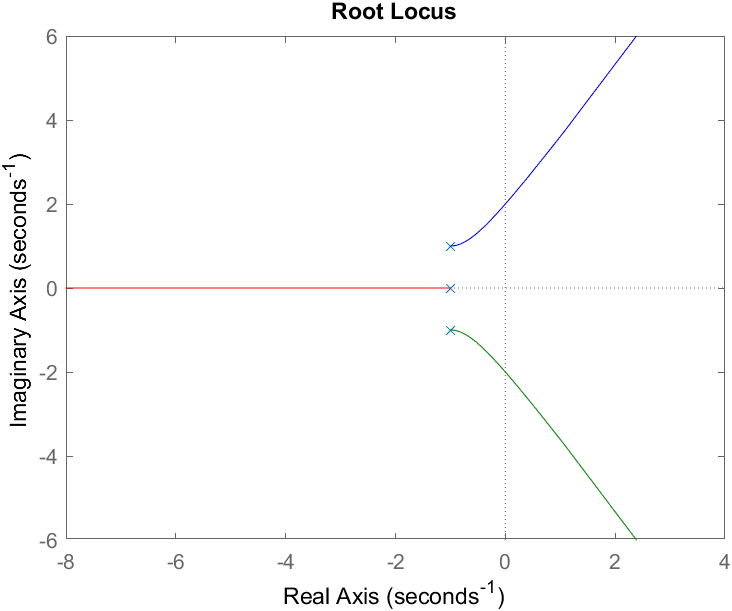
\includegraphics[width=0.35\textwidth]{AERO_422_HW5_P3b.png}
        \label{fig:P3b}
    \end{figure}
    \part[2] A closed-loop system is said to be unconditionally stable if it is stable for any $0\leq K<\infty$. Is the feedback loop under consideration unconditionally stable? Explain using root locus.\\
    \ans{No, the feedback loop is not unconditionally stable because it crosses the imaginary axis for some values of $K$. The root locus must lie exclusively in the left half-plane for the system to be unconditionally stable.}
    \part[3] Is it possible to satisfy the following performance specification on the damping ratio ($\zeta$) using the proportional-only controller that we have considered?  If yes, determine range of $K$ for which this is satisfied. (You may read approximate values from the MATLAB root locus.) If no, what would be your recommendation to satisfy this performance specification?\\
    (i) $\zeta\geq0.4$ \\
    \ans{Yes, for values of $K \leq K^*$, where $K^* \in [1.4,1.8]$}\\
    (ii) $\zeta\geq0.8$ \\
    \ans{No. Add PD controller or lead compensator to increase damping.}
\end{parts}

% \question[Bonus] In Figure \ref{fig:CLsys}, assume a proportional-only controller, i.e. $C(s)=K$. Sketch the Root Locus (by hand) for $0 \leq K < \infty$ if 
% $$ P(s) = \frac{s^2+4s+8}{s^2(s+7)} .$$
% Go through the entire seven-step process, and state the answers for each step. Do not skip
% any steps. If a step is not required, provide a complete explanation for why it does not apply.

\question[5] Suppose, in Figure \ref{fig:CLsys},
$$ P(s) = \frac{10}{(s+10)(s+1)} .$$
You have been given the following three options for the controller $C(s)$
$$C_1(s) = K_1, \quad C_2(s) = \frac{K_1s+K_2}{s}, \quad C_3(s) = \frac{K_1s^2+K_2s+K_3}{s^2}.$$
Choose the controller and determine range of controller gains that will result in a Type 1 system with a steady-state error to a unit reference ramp of less than 1/10.\\
\ans{To achieve a Type 1 system with a ramp input, we need the closed-loop transfer function to have one pole at the origin for a unity feedback system. $C_2(s)$ satisfies this requirement and will force the steady-state error to a finite value as $t$ approaches $\infty$. For us to parametrize the range of controller gains, $K_1$ and $K_2$, we need to find two constraint equations.\\\\
We have the following system transfer function: $$T(s) = \frac{Y(s)}{R(s)} = \frac{P(s)C_2(s)}{1 + P(s)C_2(s)}, \quad \text{where } r(t) = t \implies R(s) = \frac{1}{s^2}.$$ From this, we can extrapolate the transfer function for the error signal.
\begin{align*}
    E(s) &= R(s) - Y(s)\\
    &= R(s) - T(s)R(s)\\
    &= \left[1 - T(s)\right]R(s)\\
    &= \frac{s(s+1)(s+10)}{s(s+1)(s+10) + 10(K_1s + K_2)} \cdot \frac{1}{s^2}
\end{align*}
By applying the Final Value Theorem to $E(s)$, we get an expression for the steady-state error in terms of the integral gain, $K_2$. Setting this expression to meet our steady-state error criteria from the problem statement will provide us with our first gain constraint equation. $$e_{ss} = \lim_{s \to 0} s \cdot E(s) = \frac{1}{K_2} \leq \frac{1}{10}$$ $$K_2 \geq 10$$ Now we take a look at the characteristic equation of the system. $$s^3 + 11s^2 + 10s + 10(K_1s + K_2)$$ Use the Routh Stability Criterion to find the gain values that will make this system stable. This will provide us with the second constaint equation.
\begin{center}
    \begin{tabular}{ c|c c } 
        $s^3$ & $1$                           & $10(1+K_1)$\\ 
        $s^2$ & $11$                          & $10K_2$    \\ 
        $s^1$ & $\frac{110(1+K_1)-10K_2}{11}$ & 0          \\
        $s^0$ & $10K_2$                       &            \\
    \end{tabular}
\end{center}
By inspecting the Routh array, we see that the following parameters must be met to satisfy system stability: $$K_2 > 0, \quad 11(1+K_1) - K_2 > 0.$$ Therefore, the range of controller gains that will result in a Type 1 system with a steady-state error less that 1/10 to a unit reference ramp input is: $$K_2 \geq 10, \quad K_1 > \frac{1}{11}K_2 - 1.$$
}


\question[4] There exist certain rules for tuning PID controllers. These rules may provide a good starting point for tuning PID controllers for certain type of systems. Read Chapter 6: Designing PID Controllers from the class notes of Dr. DeMars (available on Canvas under supplementary material) to make yourself familiarized with such rules. 

\begin{figure}[hbt!]
    \centering
    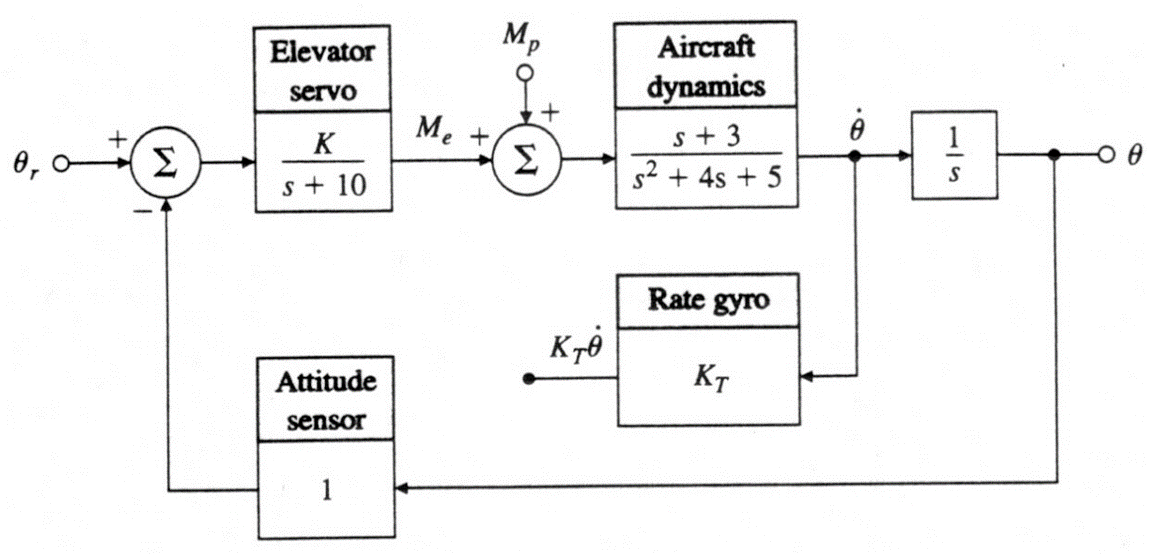
\includegraphics[width=0.75\textwidth]{AERO_422_HW5_P6.png}
    \caption{Golden Nugget autopilot}
    \label{fig:GoldenNugget}
\end{figure}

\question[Bonus] Golden Nugget Airlines has opened a free bar in the tail of their airplanes
in an attempt to lure customers. In order to automatically adjust for the
sudden weight shift due to passengers rushing to the bar when it first
opens, the airline is mechanizing a pitch-attitude auto pilot. Figure \ref{fig:GoldenNugget}
shows the block diagram of the proposed arrangement. We will model the
passenger moment as a step disturbance $Mp(s) = M_0/s$, with a maximum
expected value for $M_0$ of 0.6.
\begin{parts}
    \part[3]  What is the minimum value of $K$ is required to keep the steady-state error in $\theta$ to
    less than 0.02 rad? (Assume the system is stable.)\\
    \ans{Find the transfer function that maps the disturbance to the output. Let the elevator servo block, aircraft dynamics block, and 1/$s$ block be denoted by $C(s)$, $P(s)$, and $I(s)$, respectively. Then, $$\frac{\Theta(s)}{M_p(s)} = \frac{P(s)I(s)}{1 + P(s)C(s)I(s)}$$ Solve for $\Theta(s)$ and assume $M_p(s)$ is represented by its maximum expected value. $$\Theta(s) = \frac{\frac{s+3}{s^2 + 4s + 5} \cdot \frac{1}{s}}{1 + \frac{s+3}{s^2 + 4s + 5} \cdot \frac{K}{s + 10} \cdot \frac{1}{s}} \cdot \frac{0.6}{s} = \frac{0.6(s+3)(s+10)}{s^2(s^2 + 4s + 5)(s+10) + Ks(s+3)}$$ Find the steady-state error of the system. $$e_{ss} = \lim_{t \to \infty} \theta(t) = \lim_{s \to 0} s \cdot \Theta(s) = \lim_{s \to 0} \frac{0.6(s+3)(s+10)}{s(s^2 + 4s + 5)(s+10) + K(s+3)} = \frac{6}{K} \leq 0.02$$ Therefore, $$K \geq 300.$$}
    \part[2] Use MATLAB to draw a root locus with respect to $K$.\\
    \ans{Characteristic equation expressed in Evan's form: $$1 + K \left(\frac{s+3}{s(s^2+4s+5)(s+10)}\right) = 0$$}
    \begin{figure}[hbt!]
        \centering
        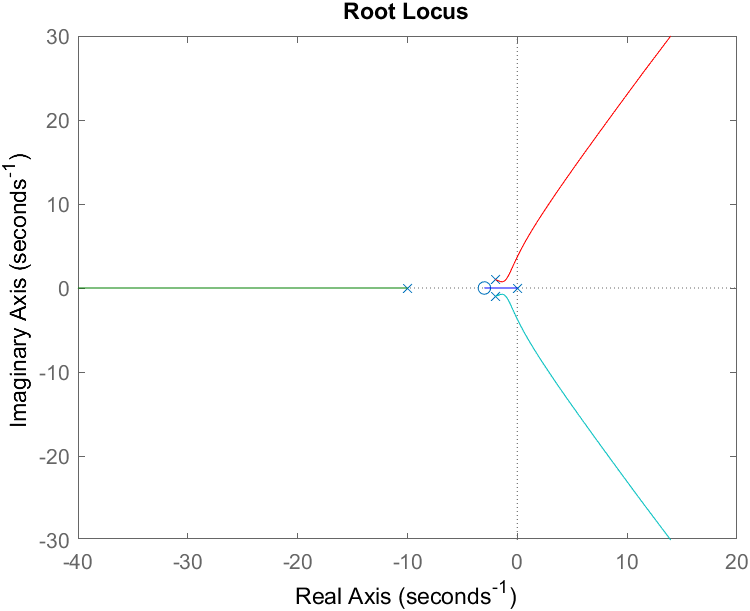
\includegraphics[width=0.45\textwidth]{AERO_422_HW5_P6b.png}
        \label{fig:P6b}
    \end{figure}
    \part[1] Based on your root locus, what is the value of $K$ when the system
    becomes unstable? (You may read an approximate value.)\\
    \ans{The system becomes unstable for $K > K^*$, where $K^* \in [130,160]$.}
    \part[2] You are given a black box with rate gyro written on the side and told
    that when installed, it provides a perfect measure of $\dot{\theta}$, with output
    $K_T\dot{\theta}$. Draw a block diagram
    indicating how you would incorporate the rate gyro into the auto pilot. (Include transfer functions in boxes.)
    \begin{figure}[hbt!]
        \centering
        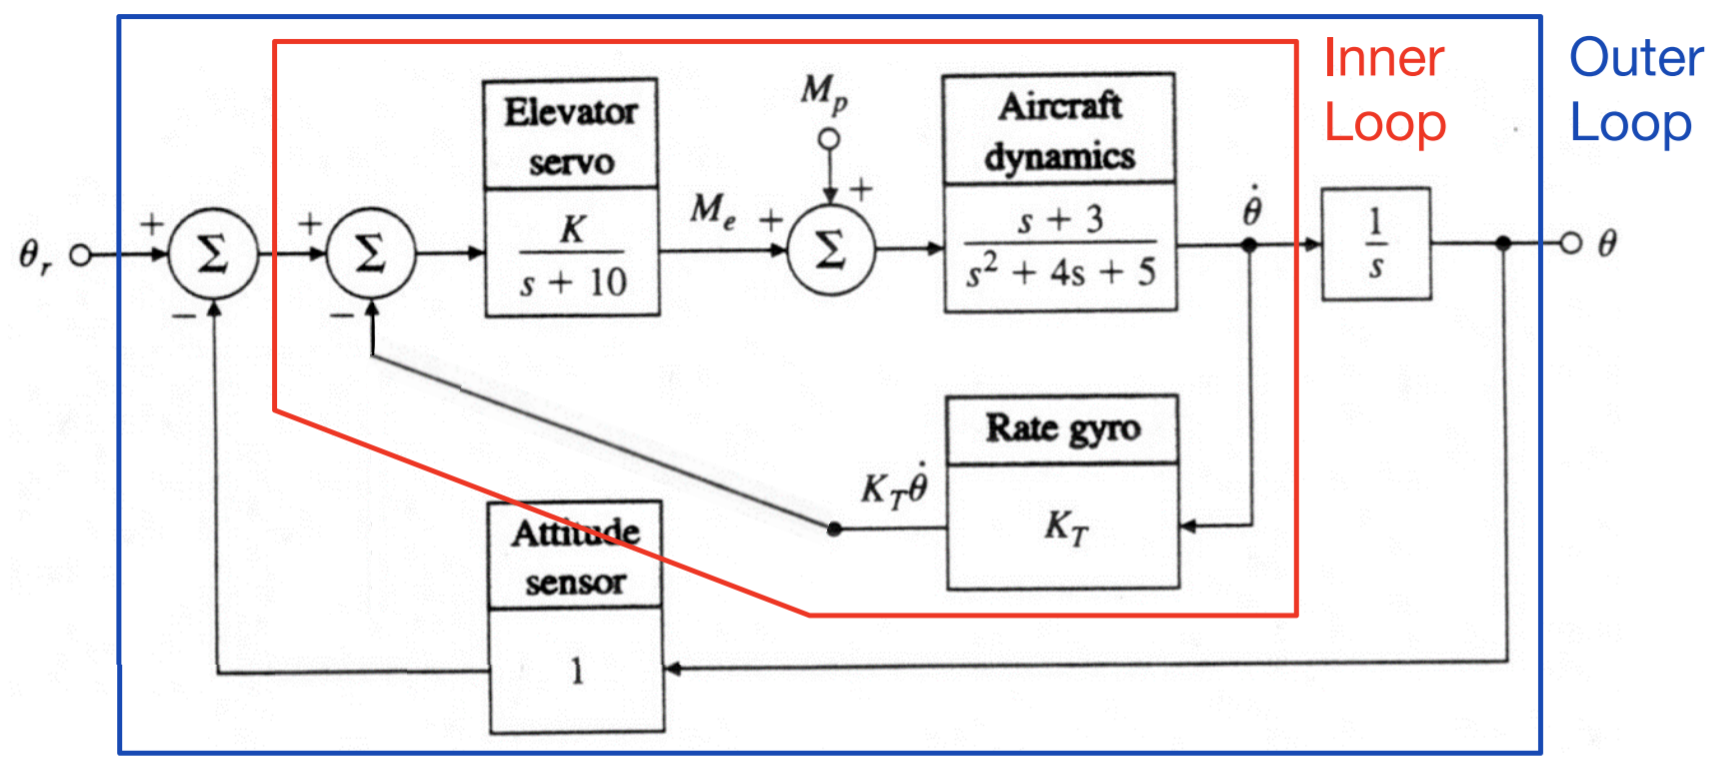
\includegraphics[width=0.8\textwidth]{AERO_422_HW5_P6d.png}
        \label{fig:P6d}
    \end{figure}
    \part[4] Assume $K = 600$ for this and the following parts of the question. Write the characteristic equation in Evans form with $K_T$ as the parameter of interest.\\
    \ans{Denote the transfer functions of the inner and outer loops by $T_1(s)$ and $T_2(s)$, respectively. $$T_1(s) = \frac{P(s)C(s)}{1 + P(s)C(s)K_T}$$ $$T_2(s) = \frac{T_1(s) \cdot I(s)}{1 + T_1(s) \cdot I(s)} = \frac{P(s)C(s)I(s)}{1 + P(s)C(s)K_T + P(s)C(s)I(s)}$$ We get the folowing characteristic equation for the outer loop: $$1 + P(s)C(s)K_T + P(s)C(s)I(s) = 0$$ Substitute $P(s)$, $C(s)$, $I(s)$, and $K = 600$ into the characteristic equation. $$1 + \frac{s + 3}{s^2 + 4s + 5} \cdot \frac{600}{s+10} \cdot K_T + \frac{s + 3}{s^2 + 4s + 5} \cdot \frac{600}{s+10} \cdot \frac{1}{s} = 0$$ Simplifying the above expression, we get $$s^4 + 14s^3 + 45s^2 + 50s + 600(s+3) + 600 K_T \left(s^2 +3s\right) = 0$$ Convert this expression into Evan's form. $$1 + K_T \frac{600 \left(s^2 +3s\right)}{s^4 + 14s^3 + 45s^2 + 650s + 1800} = 0$$}
    \part[1] Plot a root locus with respect to $K_T$.
    \begin{figure}[hbt!]
        \centering
        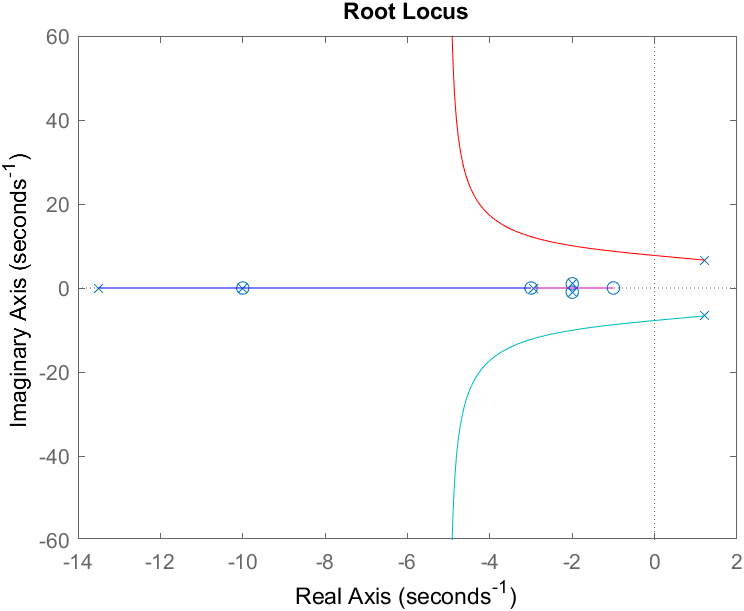
\includegraphics[width=0.45\textwidth]{AERO_422_HW5_P6f.png}
        \label{fig:P6b}
    \end{figure}
    \part[2] Considering your answers to all the previous parts, discuss the effect of rate gyro on the closed loop system.\\
    \ans{$\Theta_{ss} \leq 0.02$ requires $K \geq 300$. However, the system becomes unstable for values of $K \geq K^*$ (where $K^* \in [130,160]$). By adding a rate gyro, we are essentially adding derivative control (related to $\dot{\theta}$), thus increasing the damping ratio and increasing stability. With the addition of the rate gyro in the closed-loop system, the poles of the system can lie in the left half-plane even if $K = 600$, given appropriate values of $K_T$.}
    % \part[1] What is the maximum damping factor of the complex roots obtainable with the configuration? Comment using the root locus from previous part.
\end{parts}
\end{questions}
\end{document}